\section{Liyana Majdah Rahma(1174039)}
\subsection{Membaca ShapeFile Pyshp}
\begin{itemize}
	\item 
	\begin{figure}[H]
		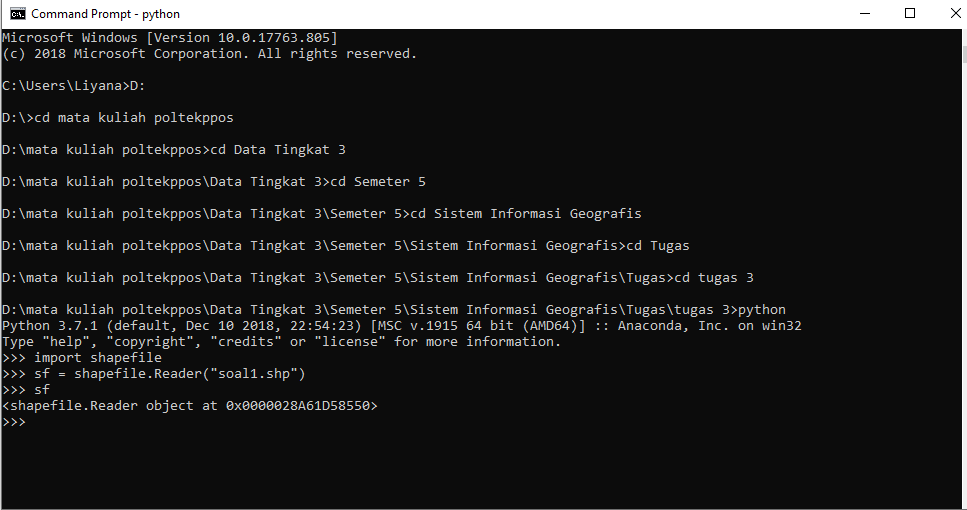
\includegraphics[width=12cm]{figures/1174039/tugas 3/hasilno1.PNG}
		\centering
		\caption{membaca file pada soal1}
	\end{figure}
	
	\item 
	\begin{figure}[H]
		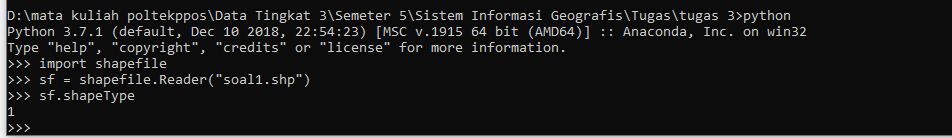
\includegraphics[width=12cm]{figures/1174039/tugas 3/hasilno2.PNG}
		\centering
		\caption{menampilkan hasil soal1 = 1}
	\end{figure}
	
	\item 
	\begin{figure}[H]
		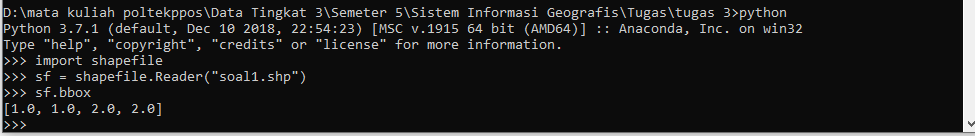
\includegraphics[width=12cm]{figures/1174039/tugas 3/hasilno3.PNG}
		\centering
		\caption{hasilnya meampilkan baris pada soal1}
	\end{figure}
	
	\item 
	\begin{figure}[H]
		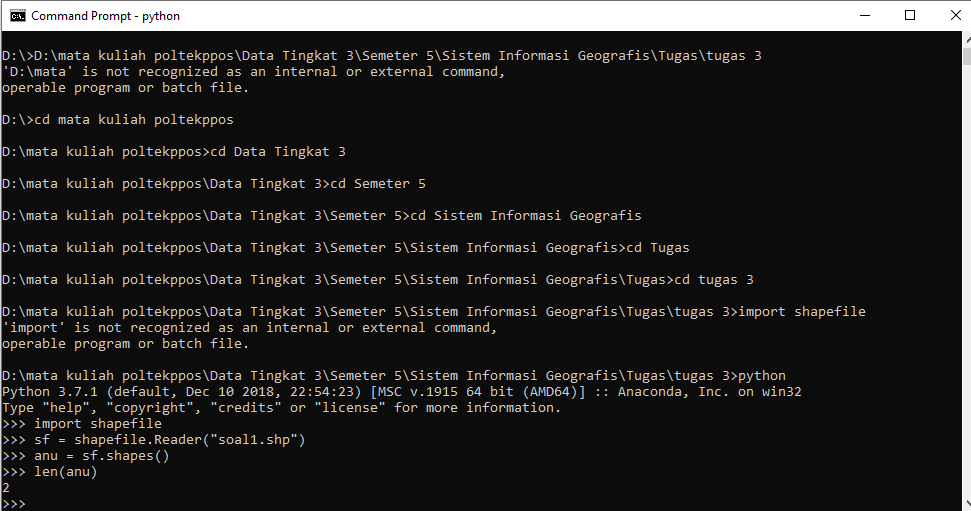
\includegraphics[width=12cm]{figures/1174039/tugas 3/hasilno4.PNG}
		\centering
		\caption{menampilkan panjang anu = 2}
	\end{figure}
	
	\item 
	\begin{figure}[H]
		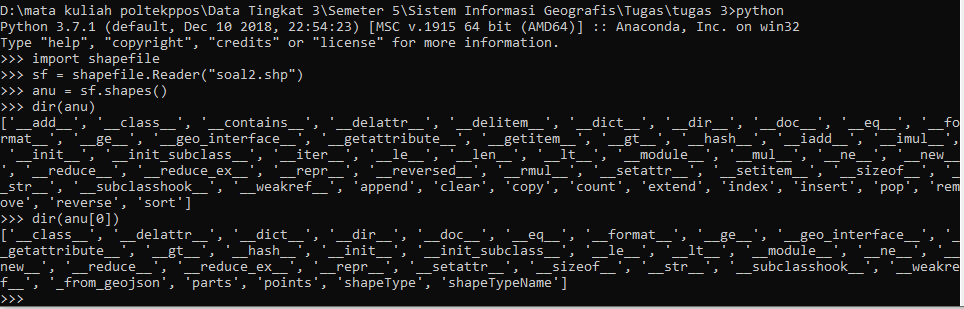
\includegraphics[width=12cm]{figures/1174039/tugas 3/hasilno5.PNG}
		\centering
		\caption{menampilkan hasil soal5}
	\end{figure}
	
	\item 
	\begin{figure}[H]
		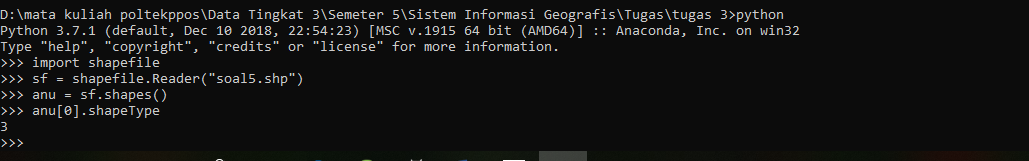
\includegraphics[width=12cm]{figures/1174039/tugas 3/hasilno6.PNG}
		\centering
		\caption{menampilkan baris pada anu = 3}
	\end{figure}
	
	\item 
	\begin{figure}[H]
		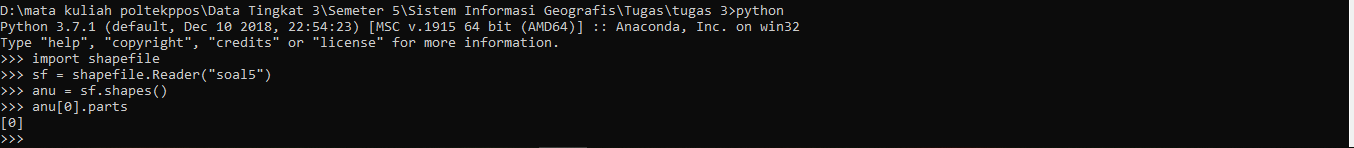
\includegraphics[width=12cm]{figures/1174039/tugas 3/hasilno7.PNG}
		\centering
		\caption{menampilkan baris pada anu}
	\end{figure}
	
	\item 
	\begin{figure}[H]
		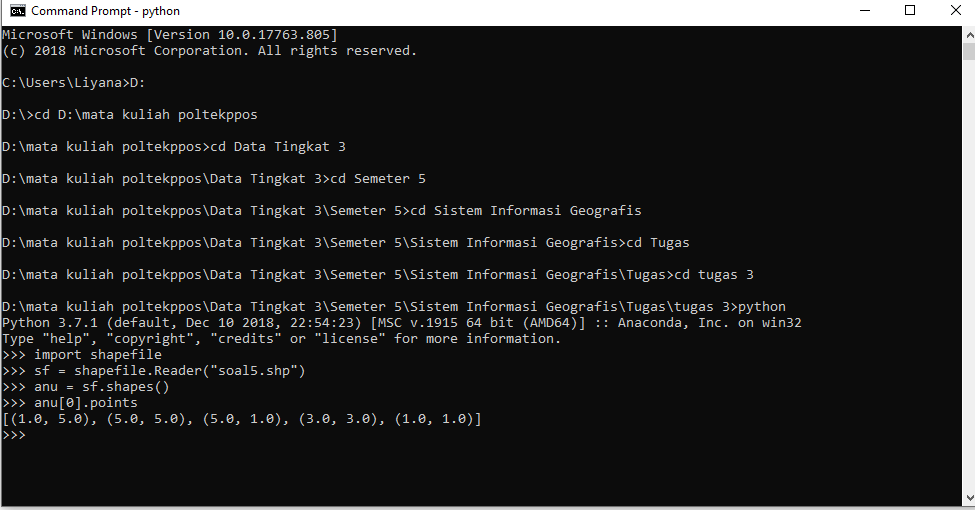
\includegraphics[width=12cm]{figures/1174039/tugas 3/hasilno8.PNG}
		\centering
		\caption{menampilkan hasil kolom dan baris pada soal5}
	\end{figure}
	
	\item 
	\begin{figure}[H]
		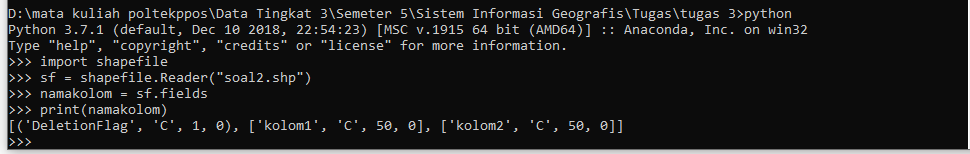
\includegraphics[width=12cm]{figures/1174039/tugas 3/hasilno9.PNG}
		\centering
		\caption{menampilkan namakolom}
	\end{figure}
	
	\item 
	\begin{figure}[H]
		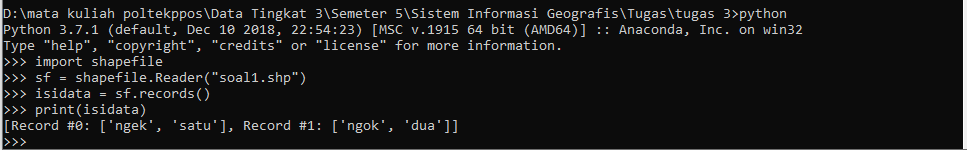
\includegraphics[width=12cm]{figures/1174039/tugas 3/hasilno10.PNG}
		\centering
		\caption{menampilkan isdata pada soal1}
	\end{figure}	

	\item 
	\begin{figure}[H]
		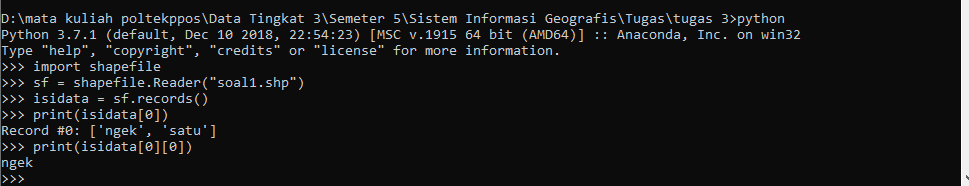
\includegraphics[width=12cm]{figures/1174039/tugas 3/hasilno11.PNG}
		\centering
		\caption{menampilkan hasil isidata record pada soal1}
	\end{figure}
\end{itemize}

\subsection{Link}
\href{https://youtu.be/pSMhSqIgpUY}{Youtube}